\documentclass[authoryear,preprint,revi	ew,12pt]{elsarticle}
\usepackage[lmargin=1in, rmargin=1in, tmargin=1in, bmargin=1in, nohead]{geometry}

\usepackage{amssymb,amsmath}
\usepackage{amsthm}
\usepackage{epsfig}
\usepackage{epsf}
\usepackage{psfrag}
\usepackage{caption}
\usepackage{latexsym, graphics, psfrag, amscd, amssymb, pb-diagram}
\usepackage{color}
\usepackage[all,cmtip]{xy}
\usepackage[lined, ruled, linesnumbered]{algorithm2e}
\usepackage{changepage}
\usepackage{tabularx ,booktabs,wrapfig,lipsum,ragged2e}
\usepackage{multirow}
\newcommand{\ra}[1]{\renewcommand{\arraystretch}{#1}}

\newtheorem{definition}{Definition}
\newtheorem{Algorithm}{Algorithm}
\newtheorem{proposition}{Proposition}
\newtheorem{theorem}{Theorem}[section]

\newcolumntype{P}[1]{>{\centering\arraybackslash}p{#1}}

\newcommand{\myvec}[1] %  {\stackrel{\raisebox{-2pt}[0pt][0pt]{\small$\rightharpoonup$}}{#1}}

\newcommand{\Eqs}     {Eqs.\ }
\newcommand{\Fig}[1]  {Fig. \ref{fig:#1}}
\newcommand{\Figs}[1] {Figs. \ref{fig:#1}}
\newcommand{\Tbl}[1]  {Table \ref{tbl:#1}}
\newcommand{\Sec}[1]  {Section \ref{sec:#1}}
\newcommand{\Secs}[1] {Sections \ref{sec:#1}}
\newcommand{\Etal}    {{\it et al}.}
\newcommand{\trans}   {\psi}
\newcommand{\acc}[1]     {$ #1 \% $}
\newcommand{\Alzheimers} {{Alzheimer\textquoteright s} }
\newcommand{\Hotellings} {{Hotelling\textquoteright s} }
\newcommand{\F}   {$ \textrm{F}_1 $}
\newcommand{\FDGPET}   {$ ^{18}\textrm{F-FDG PET} $}
\newcommand{\apoe}[1]   {Apoe$ E $#1}

% \biboptions{}

 % The \cite command functions as follows:
 %   \citet{key} ==>>                Jones et al. (1990)
 %   \citet*{key} ==>>               Jones, Baker, and Smith (1990)
 %   \citep{key} ==>>                (Jones et al., 1990)
 %   \citep*{key} ==>>               (Jones, Baker, and Smith, 1990)
 %   \citep[chap. 2]{key} ==>>       (Jones et al., 1990, chap. 2)
 %   \citep[e.g.][]{key} ==>>        (e.g. Jones et al., 1990)
 %   \citep[e.g.][p. 32]{key} ==>>   (e.g. Jones et al., p. 32)
 %   \citeauthor{key} ==>>           Jones et al.
 %   \citeauthor*{key} ==>>          Jones, Baker, and Smith
 %   \citeyear{key} ==>>             1990


\journal{Medical Image Analysis}

\begin{document}

\begin{frontmatter}

\title{3D - Patch Based Feature Extraction for Alzheimer's Disease Diagnosis via FDG-PET Analysis}

\author[asu]{Anant Srivastava}
\author[asu]{Shibani Singh}
\author[asu]{Jie Zhang}
\author[asu]{Liang Mi}
\author[Banner]{\mbox{Dhruman Goradia}}
\author[Banner]{\mbox{Kewei Chen}}
\author[Banner]{\mbox{Eric Reiman}}
\author[asu]{\mbox{Yalin Wang}\corref{cor1}}
\author{\mbox{for the Alzheimer's Disease Neuroimaging Initiative}}
\address[asu] {School of Computing, Informatics, and Decision Systems Engineering, Arizona State University, Tempe, AZ, USA}
\address[Banner] {
Banner Alzheimer's Institute, \\
Phoenix, AZ, USA}


\cortext[cor1]
{
\emph{To be submitted to Medical Image Analysis.}
\vspace{30mm}
\begin{center}
\textbf{Abstract:}  249 words\\
\textbf{Title:} 116 characters\\
\textbf{Pages:}   42 \\
\textbf{Figures:} 8 \\
\textbf{Tables:}  1\\
\vspace{10mm}
Please address correspondence to: \\
\vspace{3mm}
Dr. Yalin Wang \\
School of Computing, Informatics, and Decision Systems Engineering\\
Arizona State University\\
P.O. Box 878809 \\
Tempe, AZ 85287 USA\\
\vspace{4mm}
\textbf{Phone:} (480) 965-6871  \\
\textbf{Fax:} (480) 965-2751  \\
\textbf{E-mail:} ylwang@asu.edu
\vspace{21mm}
\end{center}
Data used in preparation of this article were obtained from the phase two of the Alzheimer\textquoteright s Disease Neuroimaging Initiative (ADNI2) database (adni.loni.usc.edu). As such, the investigators within the ADNI contributed to the design and implementation of ADNI and/or provided data but did not participate in analysis or writing of this report. A complete listing of ADNI investigators can be found at: http://adni.loni.usc.edu/wp-content/uploads/how\textunderscore to\textunderscore apply/ADNI\textunderscore Acknowledgement\textunderscore List.pdf
}

\newpage

%%%%%%%%% ABSTRACT
\begin{abstract}
Alzheimer's disease (AD), is a chronic neurodegenerative disease that usually starts slowly and gets worse over time. It is the cause of 60\% to 70\% of cases of dementia. There is growing interest in identifying brain image biomarkers that help evaluate AD risk pre-symptomatically. High-dimensional non-linear pattern classification methods have been applied to structural magnetic resonance images (MRI's) and used to discriminate between clinical groups in Alzheimer’s progression. 
Using Fluorodeoxyglucose (FDG) positron emission tomography (PET) as the preferred imaging modality, this paper develops a 3D patch based machine learning model and uses it to perform six binary classification experiments across different (AD) diagnostic categories. Specifically, from the PET image scans features were extracted and learned using probablistic PCA by taking overlapping patches in and around the cerebral cortex and using them as features. Using AdaBoost as the preferred choice of classifier both methods try to utilize \FDGPET~as a biological marker in the early diagnosis of \Alzheimers. Additional we investigate the involvement of rich demographic features (\apoe{3}, \apoe{4} and Functional Activities Questionnaires (FAQ)) in classification. The experimental results on Alzheimer's Disease Neuroimaging initiative (ADNI) dataset demonstrate the effectiveness of both the proposed systems. The paper reports a very high accuracy when comparing AD to Cognitively Normal and concludes that for least group seperation in disease progession the approach needs to be adhoc and extremely fractional. The use of \FDGPET~may offer a new sensitive biomarker and enrich the brain imaging analysis toolset for studying the diagnosis and prognosis of AD.

\end{abstract}
\begin{keyword}
Probablistic PCA, Max-pooling, Ada-boost, Alzheimer's Disease, ADNI2. 
\end{keyword}
% \PACS{PACS code1 \and PACS code2 \and more}
% \subclass{MSC code1 \and MSC code2 \and more}
\end{frontmatter}

\section{Introduction}
Alzheimer’s disease (AD) is a chronic neurodegenerative disease in which amyloid plaques and neurofibrillary tangles accumulate in the brain. The most common early symptom is the difficulty remembering recent events (short-term memory loss). As the disease advances, patients may lack motivation, have problems with self-care, and show behavioral abnormalities or even withdraw from family and society \citep{Burns2009}. AD has a typical pattern of progression, with changes in the brain that correspond to the types and severity of symptoms. Disease progression has commonly been divided into five main categories in the ADNI2 phase of Alzheimer's Disease Neuroimaging initiative(ADNI) \citep{weiner2013alzheimer}: Cognitively Normal (CN), Significant Memory Concern(SMC), Early Mild Cognitive Impairment (EMCI), Impairment (LMCI) and Alzheimer's Disease (AD), defined clinically based on behavioral and cognitive assessment. (SMC) are self-report significant memory concern from the patient we choose to exclude it from our study.

There has been a shift with a sense of urgency to find effective intervention in the presymptomatic stage of AD so to reduce the risk of AD, delay or even prevent its onset. To more adequately diagnose different stages of the disease and especially in the early stage and predict future cognitive decline, computer-aided diagnostic classification is increasingly needed using biomarkers based on neuroimaging and other measurements.
There is evidence that the pathogenic cascade of AD is thought to begin at least 1-2 decades prior to cognitive impairment, starting with accumulation of the amyloid-$\beta$1-42(A$\beta$1-42) plaques \citep{langbaum2013ushering}. Research has suggested that these early processes can be assessed using brain imaging and fluid biomarkers. Prior research work on Fluorodeoxyglucose (FDG) positron emission tomography (PET), Pittsburgh compound B (PIB), structural magnetic resonance imaging (sMRI) and functional measures of resting-state networks (rs-fMRI) has supported their validity as potential metabolic biomarkers. Among various neuroimaging techniques, \FDGPET characterizes the cerebral glucose hypometabolism related to AD and those at risk of AD. It even offers a reliable metabolic biomarker at pre-symptomatic stages. Despite major advances in FDG-PET used to track symptomatic patients, there is still a lack of sensitive, reliable, and accessible imaging algorithms capable of characterizing abnormal degrees of age-related metabolism decline in preclinical individuals at high risk for AD whom early intervention is most needed. Fig.~\ref{fig:pet_raw} shows the different types of PET scans.

Recently minor cognitive impairment (MCI) in \FDGPET ~has been classified by a brain regional sensitivity mapping method based on summated index (Total Z score) by utilizing the sensitivity-distribution maps \citep{kakimoto2011new}.In other contemporary works a region of interest (ROI) mask is used to extract features and use incomplete random forest-robust support vector machine to perform classification \citep{lu2017early}. In general for a classification algorithm based on 3D FDG-PET images the feature dimension is usually much larger than the number of subjects. Data with extremely high dimensionality has presented serious challenges to existing learning methods \citep{liu2007computational, friedman2001elements}. With the presence of a large number of features, a learning model tends to overfit, affecting its performance.

In this context, when we apply three-dimensional statistical maps to do classification the feature dimension is usually much larger than the number of subjects, i.e., the so-called “high dimension, small sample size problem”. When a vast number of variables are measured from a small number of subjects, it is often necessary to reduce their high dimension features to low dimension features. In most cases, the information gets lost by mapping into a lower-dimensional space. However, the discarding information is always compensated by a more accurate space (or feature). There are two general approaches to performing dimensionality reduction: feature selection and feature extraction. Feature selection reduces the feature dimension by selecting a subset of original variables \citep{jain1997feature}. It aims to choose a small subset of the relevant features from the original ones according to certain relevance evaluation criterion, which usually leads to better learning performance for example higher learning accuracy for classification, lower computational cost, and better model interoperability \citep{tang2014feature}. Feature extraction reduces the dimension based on mathematical projections, which transform the original features into a lower dimensional but more appropriate feature space \citep{guyon2008feature}. There are some widely used algorithms in machine learning, e.g., principle component analysis (PCA) \citep{jolliffe2002principal}, linear discriminant analysis (LDA) \citep{mika1999fisher}, as analytic tools for feature extraction.

% THIS PARA IS MORE ABOUT MATTER AND NEEDS TO BE ADDED TO THE DISCUSSION
Both Feature extraction and feature selection are capable of improving learning performance, lowering computational complexity, building better generalizable models, and decreasing required storage. Feature extraction maps the original feature space to a new feature space with lower dimensions by combining the original feature space. It is difficult to link the features from original feature space to new features. Therefore further analysis of new features is problematic since there is no physical meaning for the transformed features obtained from feature extraction techniques. While feature selection selects a subset of features from the original feature set without any transformation, and maintains the physical meanings of the original features. In this sense, feature selection is superior in terms of better readability and interpretability. This property has its significance in many practical applications such as finding relevant genes to a specific disease and building a sentiment lexicon for sentiment analysis. Typically feature selection and feature extraction are presented separately. Via sparse learning such as $\ell1$ regularization, feature extraction (transformation) methods can be converted into feature selection methods \citep{masaeli2010transformation}. In order to analyze images more efficiently, a dictionary that allows us to represent them as a superposition of a small number of its elements so that we can reduce each image to a small number of its coefficients \citep{schnass2008dictionary}. Similarly sparse coding \citep{lin2014stochastic} has been proposed to use a small number of basis vectors (also called dictionary) to represent local features effectively and concisely and help image content recognition. From the input image data, sparse coding learns an over-complete set of basis vectors (dictionary), which have been used to select the most germane features \citep*{friedman2001elements}. To learn local imaging features, image patches are usually selected to form dictionaries. Dictionary learning and sparse coding \citep{mairal2009online} has shown to be efficient for many tasks such as image deblurring \citep{yin2008bregman}, image super-resolution functional connectivity analysis \citep{lv2015holistic,lv2015modeling}, and image classification. In many computer vision, medical imaging and bioinformatics applications \citep{mairal2009online,moody2012unsupervised,lv2015modeling} dictionary learning and sparse coding leads to state-of-the-art results.

The problem of a very large set of feature with respect to sample is called ``the curse of dimensionality'' by many. To address the problem of curse of dimensionality, we propose a patch based method of data collection for PET scans and on top of that we make a layer abstracting from a probablistic machine learning model for classification for a large set of \FDGPET images, and compare its performance. The approach is a empirical machine learning based model which includes patch based feature selection then maxpooling \citep{boureau2010theoretical} for feature agglomeration. We then form data vectors and apply probabilistic principle component analysis for feature extraction using dimension reduction and finally AdaBoost \citep{rojas2009adaboost} for classification. The two systems serves as a comparison between the approaches for analyzing \FDGPET. Our goal is to discover an appropriate \FDGPET ~diagnosis system design by investigating their performance. We tested our hypothesis on the ADNI2 dataset across $668$ subjects. We then carried out 10 fold cross validation in six different classification experiments comparing the two methods across various imaging measures.

\begin{figure}[h]
	\centering
	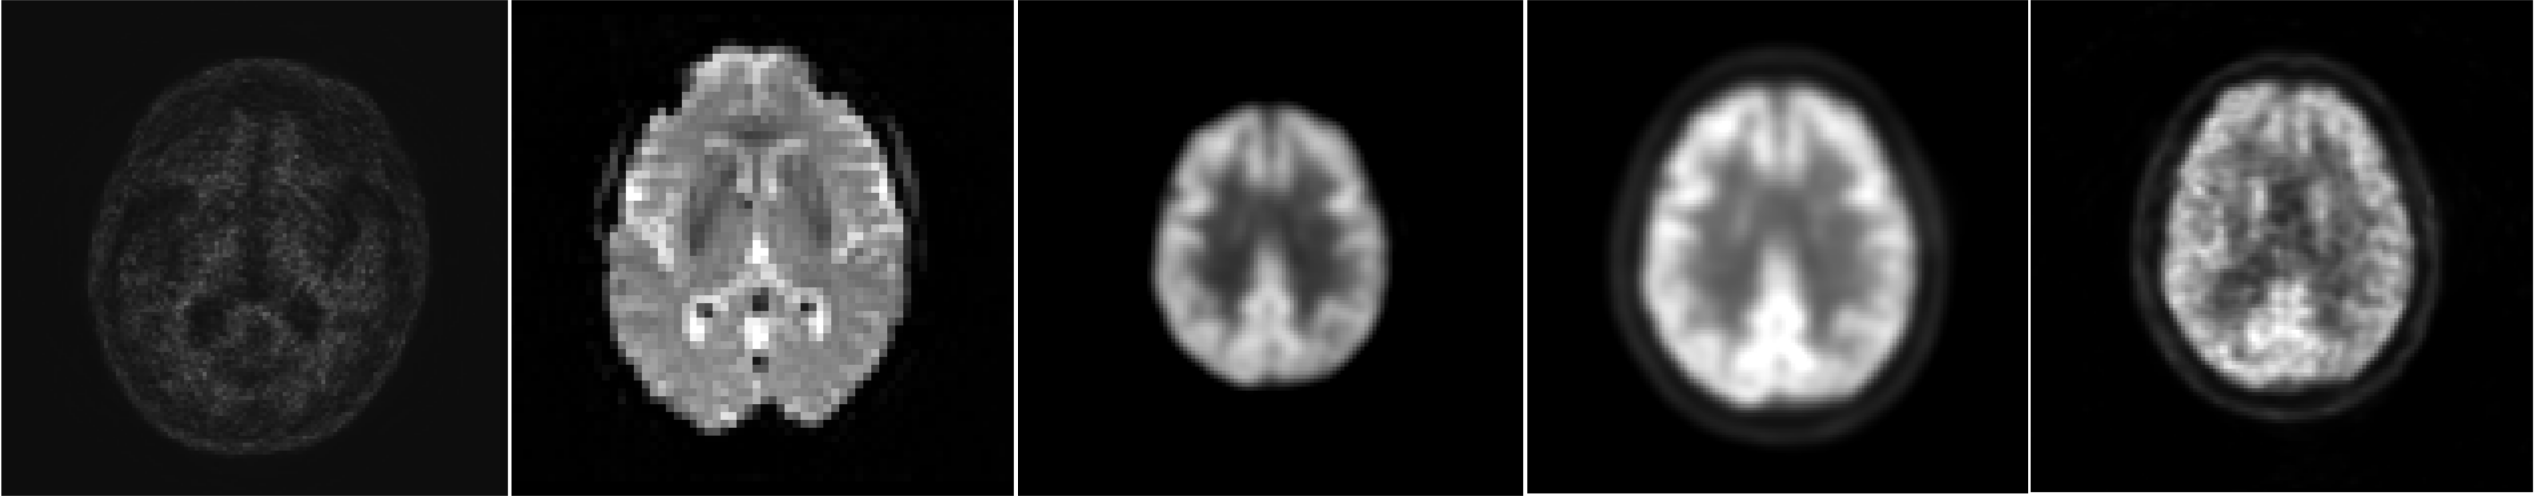
\includegraphics[width=\linewidth]{figures/pet_raw.png}
	\caption{Different types of P.E.T Scans}
	\label{fig:pet_raw}
\end{figure}	
	
\section{Methods and Material}

\subsection{Theoretical Background}
\label{subsec:theoritical_background}

% THIS PARA IS AGAIN A COMPARISION TO JIE'S PAPER MOVETO DISCUSSION
In prior work ~\cite{zhang2016applying} the authors study the surface deformation of the hippocampal region of the brain and use it as features for training a dictionary of basis vectors and associated sparse codes. This encoding learn sets of over complete basis vectors which are better able to capture structures and patterns inherent in the input data. The hippocampal surface is modeled from the hippocampal region of the brain and patches on its surface captures topological information effectively. Similar a system can be designed which uses a patch based feature extraction process and then use statistics derives form the patches for classification. However an important question for diagnostic classification based on voxel-based or surface-based maps is which statistics are best to analyze. 

% THIS PARA IS AGAIN A COMPARISION TO JIE'S PAPER MOVETO DISCUSSION
\citep{kakimoto2011new} used the total z-score from the Brodmann Area sensitivity map in the brain surface,  \citep{lu2017early} calculated the mean voxel values from 116 VOIs, standard deviations of voxel values from the 116 anatomical VOIs, and mean voxel value differences between 54 pairs of the anatomical VOIs on left and right brain hemispheres. All VOIs were extracted form a AAL template similar to the one in Fig.~\ref{fig:mask} with more regions of varying intensities. We hypothesize that a patch based extraction methods which selects overlapping volumes from each image in a number of samples and learns their reduced features can then be used for classification Algorithm.~\ref{alg:pipeline}.  

In this section, we briefly introduce the most relevant theoretical background in Dimensionality Reduction, Max-Pooling and Adaptive Boosting (AdaBoost)   

\textit{Dimension Reduction}
Feature extraction approaches project features into a new feature space with lower dimensionality and the new constructed features are usually combinations of original features. Examples of feature extraction techniques include Principle Component Analysis (PCA), Linear Discriminant Analysis (LDA) and Singular Value Decomposition(SVD). Feature extraction maps the original feature space to a new feature space with lower dimensions by combining the original feature space. In that context principle component analysis (PCA) \citep{jolliffe2002principal} is a unsupervised machine learning algorithm widely used for dimensionality reduction. It used orthogonal transformations to convert a set of observations of possibly co-related values into a set of linearly uncorrelated variables called principle components. 

After selecting the patches and structuring our 3D data into ``sample $ \times $ features'', we would wish to analyze it summarizing its main characteristics. PCA is one of the most popular techniques for processing, compressing and visualising data. We use probabilistic PCA a variation of traditional PCA to reduce the dimensions of our selected features. Traditionally PCA's effectiveness is limited by its global linearity, to overcome that a combination of local linear PCA projections has been found to be able to capture data complexity efficiently. This model variant of PCA corresponds to the probability density unlike traditional PCA and enables it to combine PCA models~ \citep{tipping1999mixtures}. After reducing the dimensions of our dataset we will classify using AdaBoost. 

\textit{Max Pooling} 
State-of-the-art patch-based image representations involve a pooling operation that aggregates statistics computed from local descriptors. After obtaining features using convolution, we would next like to use them for classification. In theory, one could use all the extracted features with a classifier such as a softmax classifier, but this can be computationally challenging. We use max-pooling which summarizes the coded features over larger neighborhoods. To address this, first recall that we decided to obtain convolved features because images have the "stationarity" property, which implies that features that are useful in one region are also likely to be useful for other regions. Thus, to describe a large image, one natural approach is to aggregate statistics of these features at various locations. If one chooses the pooling regions to be contiguous areas in the image and only pools features generated from the same (replicated) hidden units. Then, these pooling units will then be translation invariant. This means that the same (pooled) feature will be active even when the image undergoes (small) translations. Translation-invariant features are often desirable; in many tasks (e.g., object detection, audio recognition), the label of the example (image) is the same even when the image is translated. For example, if you were to take an MNIST digit and translate it left or right, you would want your classifier to still accurately classify it as the same digit regardless of its final position. Standard pooling operations include sum- and max-pooling. Sum-pooling lacks discriminability because the resulting representation is strongly influenced by frequent yet often uninformative descriptors, but only weakly influenced by rare yet potentially highly-informative ones. Max-pooling equalizes the influence of frequent and rare descriptors but is only applicable to representations that rely on count statistics, such as the bag-of-visual-words (BOV) and its soft-and sparse-coding extensions. Fig. \ref{fig:maxpooling} shows the whole process of max pooling. On the left hand side, pooling layer down-samples the volume spatially, independently in each depth slice of the input volume. On the right hand side, it is the most common max pooling shown with a stride of 2.
\begin{centering}
	\begin{figure}
		\centering
		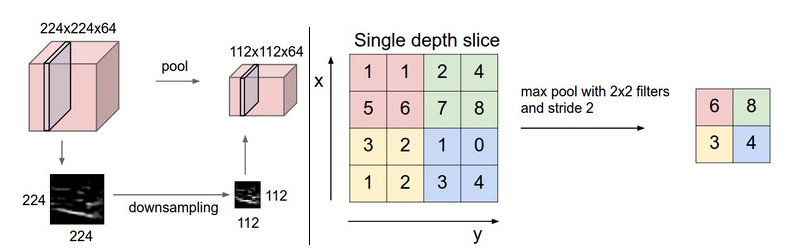
\includegraphics[width=\linewidth]{figures/maxpooling2.png}
		\caption{Pooling layer down-samples the volume spatially, independently in each depth slice of the input volume. Left: In this example, the input volume of size [256×256×16] is pooled with filter size 2; stride 2 into output volume of size [128×128×16]. Notice that the volume depth is preserved. Right: The most common down-sampling operation is max, giving rise to max-pooling, and here shown with a stride of 2, each max value is taken over 4 numbers (little 2×2 square).}
		\label{fig:maxpooling}
	\end{figure}
\end{centering}

\textit{AdaBoost}
A number of statistical classifiers have been proposed for brain biomarker research. Support vector machine and Adaptive Boosting are the most popular ones. Adaboost short for ``Abstract Boosting'' is an approach to machine learning based on the idea of creating a highly accurate prediction rule by combining many relative weak and inaccurate rules. The AdaBoost Algorithm \citep{freund1996experiments} was the first practical boosting algorithm, and remains one of the most widely used and studied, with applications in numerous fields. Adaboost can achieve more accuracy than any individual member classifier with unstable classifier. It can be used in conjunction with many other types of learning algorithms to improve their performance. One of the main ideas of the algorithm is to maintain a distribution or set of weights over the training set.  Initially, all weights are set equally, but on each round, the weights of incorrectly classified examples are increased so that the weak learner is forced to focus on the hard examples in the training set. Fig. \ref{fig:adaboost} illustrates the general idea of the AdaBoost algorithm. The algorithm takes as input a training set $ (x_1,y_1), \dots , (x_m,y_m) $ where each $ x_i $ belongs to some domain or instance space $ X $, and each label $ y_i $ is in some label set $ Y $. For most of the discussion, we assume $ Y = \{-1, +1\} $. Adaboost calls a given weak or base learning  algorithm repeatedly in a series of rounds $ t = 1,\dots,T $. One of the main ideas of the algorithm is to maintain a distribution or set of weights over the training set. The weight of this distribution on training example $ i $ on round $ t $ is denoted as $ D_t(i) $. Initially, all weights are set equally , but on each round, the weights of incorrectly classified examples are increased so that the weak learner is forced to focus on the hard examples in the training sets.
The weak learner's job is to find a weak hypothesis $ h_t : X \to \{-1 ,+1\}$ appropriate for the distribution $ D_t $. The goodness of a weak hypothesis is measured by its error.
$$ \epsilon_t = Pr_{i \sim D_t}[h_t(x_i) \neq y_i] = \underset{i:h_t(x_i) \neq y_i}{\sum} D_t(i)  $$
Notice that the error is measured with respect to the distribution $ D_t $ on which the weak learner was trained. In practice, the weak learner may be an algorithm that can use the weights $ D_t $ on the training examples. Alternatively , when this is not possible, a subset of the training examples can be sampled according to $ D_t $, and these (unweighted) resampled examples can be used to train the weak learner~\cite{schapire2013explaining}

\begin{centering}
	\begin{figure}
		\centering
		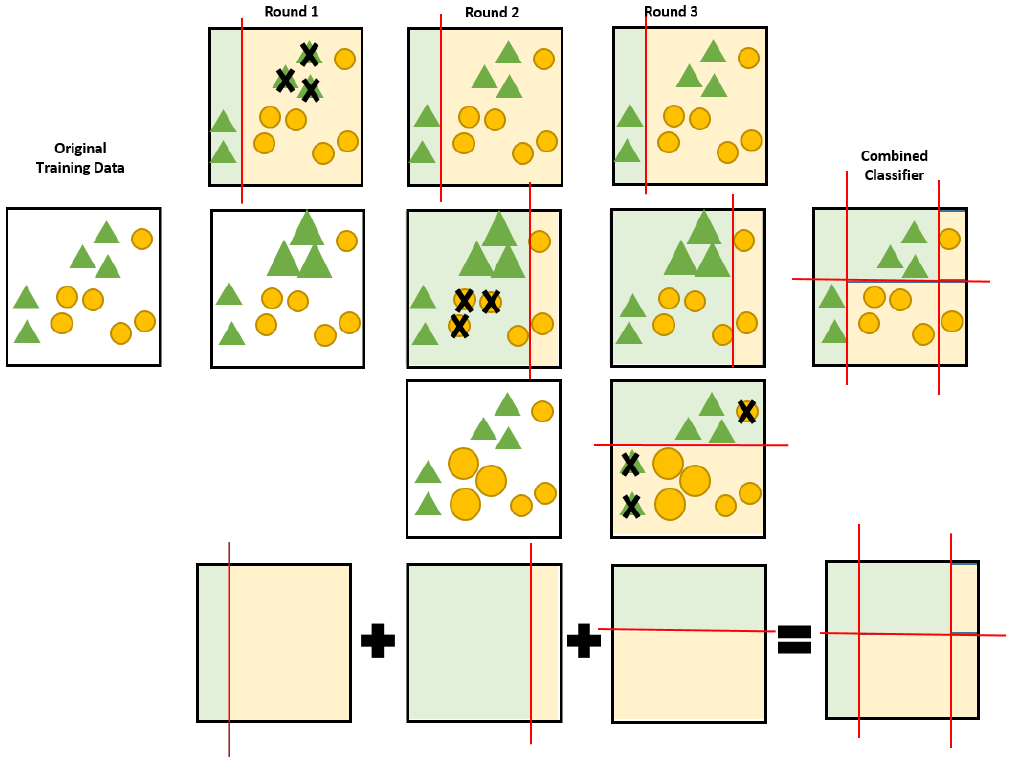
\includegraphics[width=\linewidth]{figures/adaboost.png}
		\caption[Illustration of the AdoBoost Algorithm.]{Illustration of the general idea of AdaBoost algorithm. The original training data is trained in three rounds. The first round is to create the first classifier, then the wrong classes will be given more weight and train in next round. In round 2, AdaBoost constructs a new classifier on the different weighted data. Similarly, it will give wrong classes higher weight and increase the probability of training in next round. Here, $ \times $ represents wrong classes. In the third round, AdaBoost learns a new classifier based on last round weighted data. In this figure, the bigger shape means more weight to be trained. Finally, AdaBoost combines all classifiers in three rounds (calculated in last line) into the final classifier.}
		\label{fig:adaboost}
	\end{figure}
\end{centering}

\subsection{Computational Algorithms}
\label{subsec:computational_algorithm}

This section introduces the computational algorithms of the proposed classification method in detail. Specifically, we build an integrated and automated framework to extract and analyze information from three dimensional \FDGPET~ scans, major algorithm is summarized in Alg.~\ref{alg:pipeline} and Fig.~\ref{fig:pipeline}

\subsubsection{FDG-PET acquisition and preprocessing using SPM (Statistical Parametric Mapping)}
\label{sec:preprocess}
Screening and baseline FDG-PET scans were acquired for ADNI participants included in the current study (ADNI2) project via the Image Data Archive. Scans are performed within two weeks before or two weeks after the the in-clinical assessment at Baseline. A 30-min dynamic emission scan, consisting of four 5-min frames was acquired  30 to 60 minutes post-injection. The base frame image and the five co-registered frames (or all co-registered frames for the quantitative studies) are recombined into a co-registered dynamic image set. These image sets have the same image size (for example, 128$ \times $128$ \times $63) and voxel dimensions (for example, 2.0$ \times $2.0$ \times $2.0 mm) and remain in the same spatial orientation as the original PET image data. This is called ‘native’ space. These files are uploaded to LONI in DICOM format. The scans are reoriented into a standard 160$ \times $160$ \times $96 voxel image grid having 1.5mm cubic voxels. with sections parallel to a horizontal section through the anterior and posterior commissures, normalize the images for individual variation in absolute image intensity, and apply a filter function. The images were uploaded to the Laboratory of Neuroimaging (LONI) ADNI website at UCLA and downloaded in NIFTI format.

Given a PET image, the alignment and the image segmentation are automatically performed using Statistical Parametric Mapping (SPM12) \citep{penny2011statistical}\footnote{http://www.fil.ion.ucl.ac.uk/spm/}. First, all scans are aligned to a common space. Then, we borrow a brain mask from SPM, an AAL template to decide which regions to keep and which to remove. We align the template to the same space as we did to the test images and turn the AAL template into a mask by turning all the non-zero voxels to the value of ``1''. Third we compute the dot product of the FDG-PET image scans and the mask generated to segment the region of interest. Fourth, we conduct spatial smoothing with a Gaussian kernel of the full width at half maximum (FWHM) equal to (8; 8; 8) in three directions (x; y; z).

% An illustration of the landmark curves on a left cortical surface is shown in Fig. \ref{fig:landmarks} with two views. We show the landmarks with both the original and inflated cortical surfaces for clarity.

\begin{figure}
	\centering
	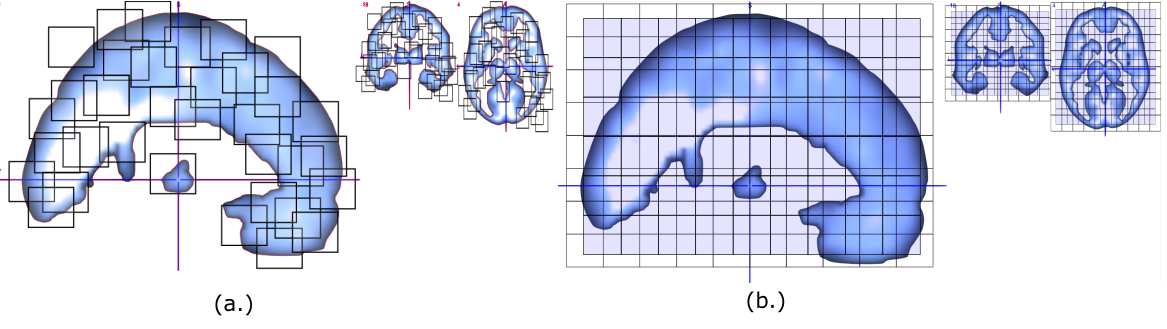
\includegraphics[width=\linewidth]{figures/patches}
	\caption[Unstructured and Structured patches in Axial, Sagittal and Coronal view of the brain.]{(a). Unstructured patches are generated randomly and ensure overlapping by creating enough of them. (b). Structured patches with overlap shown in a slightly stronger shade of blue.}
	\label{fig:patches}
\end{figure}

\subsubsection{Patch Generation and Image Representation}
\label{sec:patch_generation}
After we identify the region of interest as the cerebral cortex in the FDG-PET scans we are left with a 80 $ \times $ 95 $ \times $ 80 voxel intensities which represent the metabolic activity. For this study we choose the entire cerebral cortex as the basis for comparison or as we would call it the biomarker. The feature dimension with the FDG-PET data is much larger than the number of subjects and is therefore prone to overfitting. We first randomly generate a number of small 10 $ \times $ 10 $ \times $ 10 windows on each image volume to obtain a collection of small image patches with different amounts of overlap. The procedure is in fact equivalent to applying a high-pass filter to the original volume. As a result, the region of interest (ROI) are still present, but some low frequency signals have disappeared. 

With respect to three dimensional data one can argue as to which patch orientation and overlapping will give the best results and will not compromize the perfomance of the training algorithm. As such the processing pipeline thus has a large number of tunable parameters, such as the patch size or the orientation or even the choice of step size in the training process. It turns out that getting these parameters set correctly can make a major difference in the performance of practical applications. In fact, these parameteres have a greater contribution towards the classification performance than the training algorithm. We make two sets of patches 1.) Structured overlapping patches with uniform overlap and 2.) Unstructured overlapping patches with random overlap.

Illustration of the patch generation procedure is shown in Fig.\ref{fig:patches} (a,b). 

\subsubsection{Feature Selection and Extraction}
\label{subsec:pipline}
After we identify the region of interest as the cerebral cortex in the FDG-PET scans we are left with a 80 $ \times $ 95 $ \times $ 80 voxel intensities which represent the metabolic activity. For this study we choose the entire cerebral cortex as the basis for comparison or as we would call it the biomarker. The feature dimension with the FDG-PET data is much larger than the number of subjects and is therefore prone to overfitting. We first randomly generate a number of small 10 $ \times $ 10 $ \times $ 10 windows on each image volume to obtain a collection of small image patches with different amounts of overlap. The procedure is in fact equivalent to applying a high-pass filter to the original volume. As a result, the region of interest (ROI) are still present, but some low frequency signals have disappeared. 

In the pipeline we pool and arranged the patches into a linear array $ X_i = (x^1_i,\dots,x^n_i) $ where $ n $ is the number of feature and $ i \in \{1 \dots m\} $, where $ m $ is the number of samples in a group and stack them for the concerned group $ X = (X_1,\dots,X_i,\dots,X_m) $. The corresponding labels are also generated in this step $ Y = (y_1,\dots,y_m) $. We will then try to find out the linear and non-linear separability of the data using machine learning algorithms.

Illustration of the patch selection procedure is shown in Fig.\ref{fig:pipeline} (c).

At this step we have a good understanding of our input data for the training process, theoretically we could the data matrix $ X $ for classification. However when a vast number of variables are measured from a relatively small dataset, the feature dimension is usually much larger than the sample size and the volume of the space increases so fast that the available data becomes sparse. In such a problem an enormous amount of data is required to ensure that there are several samples with each combination of values thus ensure no overfitting. With a fixed number of training samples, the predictive power reduces as the dimensionality increases. To overcome this issue we choose to effectively represent our data by reducing the dimensions of our feature space. In machine learning, dimensionality reduction is the introduction of new feature space where the original features are represented. The new space is of lower dimension that the original space. e.g., principle component analysis (PCA) \citep{jolliffe2002principal}, linear discriminant analysis (LDA) \citep{mika1999fisher}.

 A major limitation of traditional PCA is that it is non-parametric as there is no probabilistic model for observed data. In 1999 ME Tipping \citep*{tipping1999mixtures} proposed a probabilistic PCA model (PPCA) in which the principle axes of a set of observed data vectors may be determined through maximum-likelihood estimation. The main idea of PPCA is based on the latent variable models which seeks to relate a $ d $-dimensional observed data vector $ \mathbf{t} $ to a corresponding $ q $-dimensional vector of latent variable (i.e. the unobserved variables that can be inferred from the model) $ x $.
\begin{equation}
\mathbf{y} = Wx + \mu + \epsilon
\end{equation} 
where, latent variables $ x \sim \mathcal{N}(0,I)) $. the noise model is described as $ \epsilon \sim \mathcal{N}(0,\Psi) $, and the ($ d \times q $) parameters matrix $ W $ contains the factor loading (Factor Analysis). $ \mu $ is the mean, given this formulation the observational vectors $ \mathbf{t} $ are also normally distributed $ \mathbf{t} \sim \mathcal{N}(\mu,C) $. In regards to equation (4.1) the probability model for the case of isotropic noise $ \epsilon \sim \mathcal{N}(0,\sigma^2I) $ is 
\begin{itemize}
	\item $ y|x \sim \mathcal{N}(WX + \mu, \sigma^2I) $
	\item $ y \sim \mathcal{N}(\mu, C_y) $, where $ c_y = WW^T + \sigma^2I $ (where $C_y$ is the covariance matrix for the observed data $ y $)
\end{itemize}
The Maximum Likelihood solution for PPCA is obtained as: \\$W_{MLE} = U_q(\Lambda_q - \sigma_{MLE}^2I)^{1/2}R$, \\where $U_q$ is a matrix of $q$ leading principal directions(eigen values of the covariance matrix), $\Lambda_q$ is a diagonal matrix of corresponding eigenvalues. \\$\sigma_{MLE}^2 = \frac{1}{d-q}\sum_{j=q-1}^{d}\lambda_j$ represents the variance lost in the projection and $R$ is an arbitrary $q\times q$ rotation matrix (corresponding to rotations in the latent space). 

A key motivation for this model is that because of the diagonality of $ \Psi $ (the variance not accounted by the latent factors ergo noise.) observed variables are conditionally independent given latent factors $ x $. The intention is that the dependencies between the data variables $t$ are explained by a smaller number of latent variables $x$, while $ \epsilon $ 
represents variance unique to
each observation variable, unlike PCA which treats covariance and variance similarly. 

Illustration of the PPCA is shown in Fig.\ref{fig:pipeline} (d).

The choice of classifier to process the lower dimension data is AdaBoost, as we saw in Sec.~\ref{subsec:theoritical_background} Adaboost is a good classifier for biomarker research along with Support vector matchine and a few others, we will compare Adaboost with other classifiers and prove that it is stable and robust classifier for biomarker research in the early detection of ~\Alzheimers.

\begin{algorithm}
	\vspace{1em}
	\caption{Patch Based Feature Extraction \& Dimensionality Reduction Pipeline}\label{alg:pipeline}
	
	\KwIn{A number of FDG-PET images}
	
	\KwOut{A set of features and labels for the six classification experiment}
	
	The segmented dataset is divided and segregated into 6 binary parcels.
	
	\For{exp $ \gets $ \{ [AD vs. CU], [AD vs. EMCI], [AD vs. LMCI], [CU vs. EMCI], [CU vs. LMCI], [EMCI vs. LMCI]. \}} {
		
		n $ \gets $ number of samples
		
		p $ \gets $ number of patches
		
		Initialize X = [n $ \times $ p]
		
		\For{sample $ \in $ exp}{
			A three dimensional patch of 10 $ \times $ 10 $ \times $ 10 is created in order to extract meaning full information from the 3D segmented PET scan.   
			
			A number of patches are generated over the PET volume and overlapping is ensured
			
			All patch windows are max-pooled and linearly arranged into a vector $ B $(Fig.\ref{fig:pipeline} (b)).  
			
			$ X_{sample} \gets $ B. Where sample $ \in $ m
		}
		
		In $ X $ the high dimensionality of the data is reduced by probabilistic PCA to avoid over fitting (Fig. \ref{fig:pipeline}(c)).
		
		classification of $ X $: sample $ \times $ features, $ Y $: labels, is performed by AdaBoost. 
	}
\end{algorithm}

\begin{figure}
	\centering
	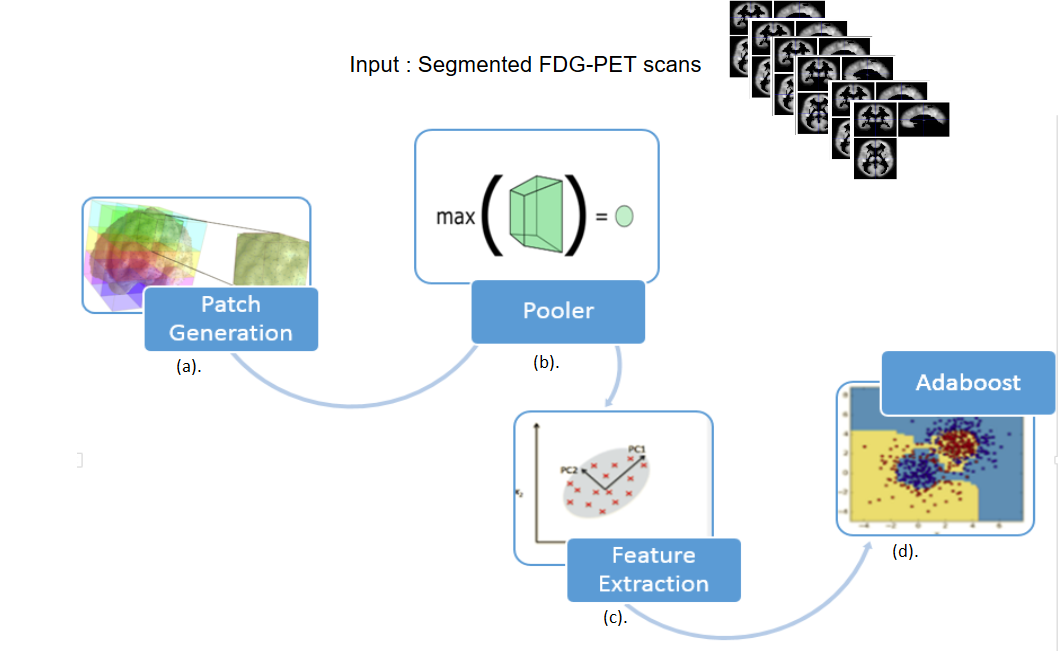
\includegraphics[width=\linewidth]{figures/pipeline2.png}
	\caption[Pipelines for Patch based Feature Extraction]{Pipelines for patch based feature extraction, (a). patches are generated for feature extraction. (b). patches are pooled to obtain specific activation. (c). the pooled values are linearly arranged and PCA is used to reduce it to a lower dimension space. (d). Adaboost is applied on the new feature space.}
	\label{fig:pipeline}
\end{figure}

\subsection{Subjects}
\label{sec:subjects}
Data used in the preparation of this article were obtained from the Alzheimer\textquoteright s Disease Neuroimaging Initiative (ADNI) database (adni.loni.usc.edu). The ADNI was launched in 2003 by the National Institute on Aging (NIA), the National Institute of Biomedical Imaging and Bioengineering (NIBIB), the Food and Drug Administration (FDA), private pharmaceutical companies and non-profit organizations, as a \$60 million, 5-year public private partnership. The primary goal of ADNI has been to test whether serial magnetic resonance imaging (MRI), positron emission tomography (PET), other biological markers, and clinical and neuropsychological assessment can be combined to measure the progression of mild cognitive impairment (MCI) and early Alzheimer\textquoteright s disease (AD). Determination of sensitive and specific markers of very early AD progression is intended to aid researchers and clinicians to develop new treatments and monitor their effectiveness, as well as lessen the time and cost of clinical trials.

The Principal Investigator of this initiative is Michael W. Weiner, MD, VA Medical Center and University of California - San Francisco. ADNI is the result of efforts of many coinvestigators from a broad range of academic institutions and private corporations, and subjects have been recruited from over 50 sites across the U.S. and Canada. The initial goal of ADNI was to recruit 800 subjects but ADNI has been followed by ADNI-GO and ADNI-2. To date, these three protocols have recruited over 1500 adults, ages 55 to 90, to participate in the research, consisting of cognitively normal older individuals, people with early or late MCI, and people with early AD. The follow up duration of each group is specified in the protocols for ADNI-1, ADNI-2 and ADNI-GO. Subjects originally recruited for ADNI-1 and ADNI-GO had the option to be followed in ADNI-2. For up-to-date information, see www.adni-info.org.

In this study, we studied a total of 668 subjects in the ADNI2 baseline dataset, within this population, there were 146 who had \Alzheimers (AD), 158 had impairment (LMCI), 178 had early mild cognitive impairment (EMCI) and 186 were normal control (CN).  


\begin{table}[t]
	\begin{center}
		\caption{Demographic Information of $668$ Subjects in the ADNI2 Baseline Dataset.}\label{tab:demographic}
		\begin{tabular}{|P{1.5cm}|P{1cm}P{1cm}P{2.25cm}P{3cm}P{1.25cm}P{1.25cm}P{1.25cm}|}
			\hline
			& Male & Female & Age & Min~/~Max Age & APOE1 & APOE2 & FAQ \\
			\hline\hline
			AD 		& $85$ 	& $61$ & $74.73 \pm 8.15$ 	& $56~/~90$ &	3.11 & 3.63 & 13.39\\
			LMCI 	& $84$ 	& $74$ & $72.5 	\pm 7.5$ 	& $55~/~91$ &	3.03 & 3.54 & 03.62\\
			EMCI 	& $102$ & $76$ & $ 71.3 \pm 7.2 $	& $55~/~89$ &	2.94 & 3.42 & 02.08\\
			CN 		& $89$ 	& $97$ & $ 73.5 \pm 6.25 $ 	& $57~/~89$ &	2.86 & 3.24 & 00.16\\
			\hline
		\end{tabular}
	\end{center}
\end{table}


\section{Experimental Results}
\label{sec:results}
We design six experiments (1). AD vs. CU (2). AD vs. EMCI (3). AD vs. LMCI (4). CU vs. EMCI (5). CU vs. LMCI (6). EMCI vs. LMCI. The objective here is to independently study the inter-cohort relationships in hope of learning more about the class separation in AD clinical group.

We run the six experiments over the pipeline described in Algorithm~\ref{alg:pipeline}. An N-fold cross validation protocol was adopted to estimate classification accuracy. All subjects were randomly divided into N folds. The surface biomarkers were selected by training on N-1 folds and the test was performed on the remaining fold. We rotated this procedure for N times to estimate the accuracy. In this paper, we choose N = 10 to complete the classification.The output of each classification experiment was compared to the ground truth, and a contingency table was computed to indicate how many class labels were correctly identified as members of one of the two classes. The rows of the contingency table represent the true classes and the columns represent the assigned classes. The cell at row r and column $c$ is the number of subjects whose true class is r while their assigned class is $c$. Natural performance measures for classification problems mainly based on error rate or accuracy. However, higher accuracy does not necessarily imply better performance on target task. In two-category classification, one method for handling $c$-class problem is to consider $c$ 2-class problems: $ \frac{\omega_i}{not ~\omega_i} $ \citep{fawcett2004roc}. Therefore, confusion matrix was proposed as a method to measure classifier performance. TP, FP, TN, FN represents number of true positives, number of false positives, number of true negatives and number of false negative, respectively. The matrix in Table.~\ref{tab:confusion_matrix} represents a possible combination of ground truth and predicted classification for two classes.

\begin{table}[]
	\centering
	\begin{tabular}{|P{3.5cm}|P{3.5cm}|P{3.5cm}|}
		\hline
		& \multicolumn{2}{|P{7cm}|}{\emph{\bf Assigned Class}}\\
		\hline
		\emph{\bf True Class}& Positive & Negative \\
		\hline
		Positive & TP & FP \\
		Negative & FN & TN \\	
		\hline
	\end{tabular}
	\caption{The Confusion Matrix}
	\label{tab:confusion_matrix}
\end{table}

The total of TP, FP, FN, TN refers to the total number in the classification. Five performance measures \F~Score, Recall, Specificity, Positive predictive value and Negative predictive value were calculated as follows:

\begin{equation*}
\textrm{F}_1~\textrm{Score} = 2 \times \frac{\textrm{TP}}{\textrm{FN} + 2\times \textrm{TP} + \textrm{FP}}.
\end{equation*}

In a given population precision measures the amount of true cases classified correctly and recall the strength of that number. When you have both high precision and high recall it would mean that the population is well classified. \F~Score is the measure that is the harmonic mean of precision and recall. The reason for taking harmonic mean is because it is more appropriate when dealing rates and ratios.  

\begin{equation*}
\textrm{Recall} = \frac{\textrm{TP}}{\textrm{TP} + \textrm{FN}}.
\end{equation*}

Recall in this context is also referred as the true positive rate or sensitivity.  is a statistical measure of how well a binary classification test correctly identifies a condition and the probability of correctly labeling members of the target class.

\begin{equation*}
\textrm{Specificity} = \frac{\textrm{TN}}{\textrm{FP} + \textrm{TN}}.
\end{equation*}

The specificity is a statistical measure of how well a binary classification test correctly identifies the negative cases.

\begin{equation*}
\textrm{Positive predictive value} = \frac{\textrm{TP}}{\textrm{TP} + \textrm{FP}}.
\end{equation*}

Where positive predictive value (PPV) is also referred to as precision, which measures the probability of a positive prediction is correct.

\begin{equation*}
\textrm{Negative predictive value} = \frac{\textrm{TN}}{\textrm{TN} + \textrm{FN}}.
\end{equation*}

which measures the probability of a negative prediction is correct.

All these measures provide relevant information about the classification and no single measure tells the entire story. For example consider a scenario where 90\% of the population does not have a disease and the 10\% population is misclassified by the classifier, the accuracy would still be 90\%. Thus we should use multiple measures.   

There are some standard performance evaluation measures for classification study. Bigger values usually mean stronger classification power. We also computed the area-under-the-curve (AUC) of the receiver operating characteristic (ROC). The ROC is the average value of sensitivity for all the possible values of specificity. Such an index is especially useful in a comparative study of two diagnostic tests. If two tests are to be compared, it is desirable to compare the entire ROC curve rather than at a particular point \citep{swets1979roc}. The maximum AUC=1 means that the diagnostic test is perfect in the differentiation between the diseased and stable. This happens when the distribution of test results for the diseased and stable do not overlap. AUC = 0.5 means the chance of discrimination that curve located on diagonal line in ROC space. 

% 1. variety of features
% 2. comparing fearure learning algorithms 
% 3. comparing classifiers 
% 4. comparing dimensionality reduction w/t sparse coding 
% 5. comparing DTI data with proposed pipeline
% 6. compare with a state of the art result.

\subsection{Variety of Features}
\label{subsection:feature_comp}
In the training matrix we then involve additional features which enables us to make well defined classification, we include the genetic information and Functional Activities Questionnaire (FAQ) Scores even Age and Gender were involved. the two alleles of Apolipoprotein E(APOE) are available, APOE genotype is represented by combination of $e2$ (episilon 2),$e3$ and $e4$. Each individual will have one of the following combinations: $e2/e2$, $e2/e34$, $e2/e44$, $e3/e3$, $e3/e4$, $e4/e4$. Although the order between two genotypes for each person doesn't matter, they are represented in the order of $e2 \ge e3 \ge e4$. After feature annotation, the dimension of the dataset was reduced to a reasonable size and classification was performed.

We ran the pipeline in Sec.~\ref{sec:pipline} over 1.) Voxels information 2.) Voxel information and genetic scores 3.) Voxel, genetic scores and other demographic information. The results of the experiment are shown Table.~\ref{tab:feature_comp} 

\begin{table}[!h]
	\centering
	\begin{tabular}{|P{3cm}|P{3cm}P{2cm}P{3cm}|}
		\hline
		Exp.& Voxels & Voxels + Gene + FAQ &  Voxels + Gene + FAQ + Demo\\\hline
		AD vs. CU		&$ 88.97 $&$ 95.10  $&$ 96.30 $\\
		AD vs. EMCI 	&$ 76.92 $&$ 81.69 $&$ 83.68 $\\
		AD vs. LMCI		&$ 63.26 $&$ 69.44 $&$ 73.42 $\\
		CU vs. EMCI		&$ 54.49 $&$ 62.63 $&$ 69.94 $\\
		CU vs. LMCI		&$ 63.87 $&$ 82.19 $&$ 78.28 $\\
		EMCI vs. LMCI	&$ 58.04 $&$ 59.47 $&$ 57.38 $\\
		\hline
	\end{tabular}
	\caption[Comparison Results between Sets of Features]{Comparison results between different sets of features. The measure used in F1-Score, three different sets of features are used to compare the effectiveness of Voxel, ~\apoe{1},~\apoe{2}, FAQ and age/gender in classification.}
	\label{tab:feature_comp}
\end{table}

It is clear from the Table.~\ref{tab:feature_comp} that the combination of voxel information and other genetic and demographic features gives the best classification result. The groups with high class seperation AD vs. CU has the maximum F-1 score of $ \sim 96 \% $. 

\subsection{Comparing Fearure learning algorithms}
\label{subsection:dim_red}
We wonder how other dimension reduciton algorithms react to our method, we compare probablistic PCA with frequently used learning methods such as linear Singular Valued Decomposition and non linear Kernel-PCA.
As indicated in Table.~\ref{tab:comparision_dimension_reduction} the \F~Score of AD vs CU is best when the dimensions are reduced using singular valued decomposition (SVD) with \acc{97} \F~Score. The high Recall and Specificity implies AD vs CU is well classified. Again we believe the \FDGPET~biomarker along with \apoe{2} and \apoe{3} the two alleles of Apolipoprotein E and the Functional Activities Questionnaire (FAQ) are extremely sensitivity if classifying between \Alzheimers and Normal Control. 
Column two in Table.\ref{tab:comparision_dimension_reduction} shows that the subjects in AD vs EMCI are separable to a good extent with \F~Score of \acc{83.3} in case of Principle Component Analysis (PCA) and a Recall of \acc{84.5} and Specificity of \acc{85.7} shows that both the classes have been evenly separated. 
Kernel PCA \citep{mika1998kernel} performed the best in remaining experiments. With CU vs LMCI the group separation is of one i.e. the disease progression there is one stage in between CU and LMCI and we observe in column 5 of Table.~\ref{tab:comparision_dimension_reduction} the \F~Score is \acc{80}. With AD vs LMCI and CU s EMCI with Kernel PCA the \F~Score is \acc{76.65} and \acc{71.46} respectively. The last experiment (LMCI vs EMCI) \F~Score of \acc{60.3} is the most difficult to classify many good and popular classifiers failed to classify the complex nature of early Mild impairment (EMCI) and impairment (LMCI). EMCI and LMCI as described in Section~\ref{subjects} are derived from the Mild Cognitive Impairment (MCI) stage in ADNI1 and the participants reported a subjective memory concern the difference in EMCI and LMCI is decided by the Wechsler Memory Scale Logical (WMS). We believe there is no clear separation with \FDGPET~ as our biomarker and maybe more specific ROI may lead us to a more concrete conclusion. 

\begin{table}[]
	\centering
	\begin{tabular}{|P{2.25cm}|P{2.5cm}P{1.25cm}P{1.25cm}P{1.25cm}P{1.25cm}P{1.25cm}P{1.25cm}|}
		\hline
		Measure&Method& AD \ CU & AD \ EMCI & AD \ LMCI & CU \ EMCI & CU \ LMCI & LMCI \ EMCI \\\hline
		\multirow{5}{*}{PCA}
		& F1 Score		&$ 96.85 $&$ 83.33 $&$ 73.42 $&$ 69.94 $&$ 78.28 $&$ 57.38 $\\
		& Recall		&$ 94.38 $&$ 84.50 $&$ 75.00 $&$ 67.50 $&$ 78.07 $&$ 58.04 $\\
		& Specificity	&$ 99.26 $&$ 85.71 $&$ 75.00 $&$ 58.90 $&$ 74.52 $&$ 52.46 $\\
		& PPV			&$ 99.46 $&$ 82.19 $&$ 71.91 $&$ 72.58 $&$ 78.49 $&$ 56.74 $\\
		& NPV			&$ 92.46 $&$ 87.64 $&$ 77.85 $&$ 63.48 $&$ 74.40 $&$ 53.79 $\\
		\midrule
		\multirow{5}{*}{SVD}
		& F1 Score		&$ 97.09 $&$ 81.85 $&$ 70.23 $&$ 66.67 $&$ 77.62 $&$ 57.47 $\\
		& Recall		&$ 95.33 $&$ 85.18 $&$ 68.62 $&$ 67.78 $&$ 77.83 $&$ 58.82 $\\
		& Specificity	&$ 98.56 $&$ 83.59 $&$ 72.19 $&$ 65.59 $&$ 73.58 $&$ 53.01 $\\
		& PPV			&$ 98.92 $&$ 78.76 $&$ 71.91 $&$ 65.59 $&$ 77.41 $&$ 56.17 $\\
		& NPV			&$ 93.83 $&$ 88.76 $&$ 69.62 $&$ 67.41 $&$ 74.05 $&$ 55.69 $\\	
		\midrule
		\multirow{5}{*}{Kernel PCA}
		& F1 Score		&$ 96.65 $&$ 82.47 $&$ 76.65 $&$ 71.46 $&$ 80.01 $&$ 60.39 $\\
		& Recall		&$ 95.77 $&$ 82.75 $&$ 78.01 $&$ 68.47 $&$ 78.06 $&$ 59.56 $\\
		& Specificity	&$ 96.50 $&$ 85.47 $&$ 77.91 $&$ 70.80 $&$ 77.02 $&$ 54.90 $\\
		& PPV			&$ 97.31 $&$ 82.19 $&$ 75.34 $&$ 74.73 $&$ 82.25 $&$ 61.23 $\\
		& NPV			&$ 94.52 $&$ 85.95 $&$ 80.37 $&$ 64.04 $&$ 72.78 $&$ 53.16 $\\
		\hline
	\end{tabular}
	\caption[Classification Results with PCA, SVD and Kernel PCA]{Classification Results with PCA, SVD and Kernel PCA. In this comparison we used Adaboost as a fixed classifier for all the reduction technique.}
	\label{tab:comparision_dimension_reduction}
\end{table}


\subsection{Comparing Classifiers}
\label{subsection:classifier_comp}
To demonstrate the effectiveness of AdaBoost as a good classifier for biomarker related research in \Alzheimers classification we compare nine classifiers and report the best four as illustrated in Table.~\ref{tab:comparision_classifiers}. The \F~Score of AD vs CU is best for Gaussian Process (GP) with a $ 97.3 \% $ \F~Score compared to $ 96.2 \% $ in AdaBoost. $ 98.38 \% $ PPV and $ 95.20 \% $ NPV indicates both the classes have been effectively classified. The class separation is maximum in case of AD vs CU in reference to disease progression that explains the high \F measure. For AD vs EMCI, AD vs LMCI, CU vs EMCI and CU vs LMCI the \F Score is highest case of Gaussian Process. In case of CU vs LMCI AdaBoost performs comparatively poor in comparison to other classifiers. For EMCI vs LMCI the NPV is poor for GP and Linear SVM which means one class is poorly classifier and the classification accuracy is inconsistent. In this case AdaBoost performed good as it gave a more consistent NPV and PPV the recall and sensitivity is also the best in this experiment. For further comparison between dimensionality reduction we keep our classifier as AdaBoost because of a more correct classification when AdaBoost was used as classifier across all the experiments.
\clearpage

\begin{table}[!h]
	\centering
	\begin{tabular}{|P{3cm}|P{2.5cm}P{1.25cm}P{1.25cm}P{1.25cm}P{1.25cm}P{1.25cm}P{1.25cm}|}
		\hline
		Measure&Method& AD \ CU & AD \ EMCI & AD \ LMCI & CU \ EMCI & CU \ LMCI & LMCI \ EMCI \\\hline
		\multirow{4}{*}{Nearest Neighbor}
		& F1 Score		&$ 96.53 $&$ 83.33 $&$ 75.98 $&$ 73.65 $&$ 84.87 $&$ 60.77 $\\
		& Recall		&$ 95.76 $&$ 88.46 $&$ 79.69 $&$ 67.41 $&$ 77.67 $&$ 56.52 $\\
		& Specificity	&$ 96.50 $&$ 84.02 $&$ 76.60 $&$ 75.00 $&$ 90.00 $&$ 52.71 $\\
		& PPV			&$ 97.31 $&$ 78.76 $&$ 72.60 $&$ 81.18 $&$ 93.54 $&$ 65.73 $\\
		& NPV			&$ 94.52 $&$ 91.57 $&$ 82.91 $&$ 58.98 $&$ 68.35 $&$ 43.03 $\\
		\midrule
		\multirow{4}{*}{Linear SVM}
		& F1 Score		&$ 96.79 $&$ 83.27 $&$ 77.35 $&$ 75.79 $&$ 84.95 $&$ 67.27 $\\		
		& Recall		&$ 96.27 $&$ 86.67 $&$ 78.72 $&$ 65.87 $&$ 77.43 $&$ 56.75 $\\
		& Specificity	&$ 96.52 $&$ 84.65 $&$ 78.52 $&$ 82.14 $&$ 90.67 $&$ 59.74 $\\
		& PPV			&$ 97.31 $&$ 80.13 $&$ 76.02 $&$ 89.24 $&$ 94.08 $&$ 82.58 $\\
		& NPV			&$ 95.20 $&$ 89.88 $&$ 81.01 $&$ 51.68 $&$ 67.72 $&$ 29.11 $\\
		\midrule
		\multirow{4}{*}{Gaussian Process}
		& F1 Score		&$ 97.34 $&$ 83.68 $&$ 77.58 $&$ 75.96 $&$ 85.64 $&$ 63.76 $\\
		& Recall		&$ 96.31 $&$ 86.76 $&$ 80.74 $&$ 68.69 $&$ 79.35 $&$ 55.93 $\\
		& Specificity	&$ 97.88 $&$ 85.10 $&$ 78.10 $&$ 79.10 $&$ 89.68 $&$ 54.00 $\\
		& PPV			&$ 98.38 $&$ 80.82 $&$ 74.65 $&$ 84.94 $&$ 93.01 $&$ 74.15 $\\		
		& NPV			&$ 95.20 $&$ 89.88 $&$ 83.54 $&$ 59.55 $&$ 71.51 $&$ 34.17 $\\		
		\midrule
		\multirow{4}{*}{AdaBoost}
		& F1 Score		&$ 96.85 $&$ 83.33 $&$ 73.42 $&$ 69.94 $&$ 78.28 $&$ 57.38 $\\
		& Recall		&$ 94.38 $&$ 84.50 $&$ 75.00 $&$ 67.50 $&$ 78.07 $&$ 58.04 $\\
		& Specificity	&$ 99.26 $&$ 85.71 $&$ 75.00 $&$ 58.90 $&$ 74.52 $&$ 52.46 $\\
		& PPV			&$ 99.46 $&$ 82.19 $&$ 71.91 $&$ 72.58 $&$ 78.49 $&$ 56.74 $\\
		& NPV			&$ 92.46 $&$ 87.64 $&$ 77.85 $&$ 63.48 $&$ 74.40 $&$ 53.79 $\\				
		\hline
	\end{tabular}
	\caption[Classification Results between Classifiers using Feature Extraction]{Classification results between different classifiers. Popular classifiers are used to perform analysis on the best feature set.}
	\label{tab:comparision_classifiers}
\end{table}

\subsection{Comparing Dimensionality Reduction with Sparse Coding}
\label{subsection:method_comp}
This experiment further investigates what if some other feature learning method is used insted of dimensionality reduction. Sparse coding has been applied in many fields like audio processing, text mining and image recognition, Sparse coding concerns the problem of reconstruting data vectors using sparse combination of basis vectors. \citep{lin2014stochastic,olshausen1996emergence}. We report the variation in the results in Figure.~\ref{tab:dim/SC}.

\begin{table}[!h]
	\centering
	\begin{tabular}{|P{3cm}|P{2.5cm}|P{1.25cm}P{1.25cm}P{1.25cm}P{1.25cm}P{1.25cm}P{1.25cm}|}
		\hline
		Measure & Method & AD \ CU & AD \ EMCI & AD \ LMCI & CU \ EMCI & CU \ LMCI & LMCI \ EMCI \\\hline
		\multirow{2}{*}{F1 Score}		
		& FE  &$ 96.53 $&$ 83.33 $&$ 75.98 $&$ 73.65 $&$ 84.87 $&$ 60.77 $\\\cline{2-2}
		& SCC &$ 96.53 $&$ 83.33 $&$ 75.98 $&$ 73.65 $&$ 84.87 $&$ 60.77 $\\
		\midrule
		\multirow{2}{*}{Recall}			
		& FE &$ 95.76 $&$ 88.46 $&$ 79.69 $&$ 67.41 $&$ 77.67 $&$ 56.52 $\\\cline{2-2}
		& SCC &$ 95.76 $&$ 88.46 $&$ 79.69 $&$ 67.41 $&$ 77.67 $&$ 56.52 $\\
		\midrule
		\multirow{2}{*}{Specificity} 	
		& FE &$ 96.50 $&$ 84.02 $&$ 76.60 $&$ 75.00 $&$ 90.00 $&$ 52.71 $\\\cline{2-2}
		& SCC &$ 95.76 $&$ 88.46 $&$ 79.69 $&$ 67.41 $&$ 77.67 $&$ 56.52 $\\
		\midrule	
		\multirow{2}{*}{PPV}		
		& FE &$ 97.31 $&$ 78.76 $&$ 72.60 $&$ 81.18 $&$ 93.54 $&$ 65.73 $\\\cline{2-2}
		& SCC &$ 95.76 $&$ 88.46 $&$ 79.69 $&$ 67.41 $&$ 77.67 $&$ 56.52 $\\
		\midrule
		\multirow{2}{*}{NPV}					
		& FE &$ 94.52 $&$ 91.57 $&$ 82.91 $&$ 58.98 $&$ 68.35 $&$ 43.03 $\\\cline{2-2}	
		& SCC &$ 95.76 $&$ 88.46 $&$ 79.69 $&$ 67.41 $&$ 77.67 $&$ 56.52 $\\
		\hline
	\end{tabular}
	\caption[Classification Results between Classifiers using Feature Extraction]{Classification results between different classifiers. Popular classifiers are used to perform analysis on the best feature set.}
	\label{tab:dim/SC}
	\end{table}

Area under the Curve is used to measure receiver operating characteristic (ROC) curve. The area is a measure of the predictive power of the classification experiment to classify a  randomly chosen positive example more accurately than a randomly chosen negative example. ROC is the graphical plot between the true positive rate and the false positive rate, it was first used during World War 2 for detecting enemy objects from friendly ships and noise. Know as Signal detection theory, it measures the ability of radar receiver operators to identify enemy ships.

Fig.~\ref{fig:auc} illustrates the classification in all clinical groups with different features performance comparison with receiver operating characteristic (ROC) curves and area under curve (AUC) measures. The results for Patch based Feature Extraction (PFE) and Patch based Feature Extraction (PFE)  with other demographic features are computed with the proposed pipeline in Alg.\ref{alg:pipeline}, patch based Dictionary Learning (PDL) is applied to dataset before training as described in Alg Alg.\ref{alg:piplinecompare}. Within the four statistics, the result of using Feature Extraction with Voxles, APOE and FAQ are better than others. Among all AUC measures, PFE+Demo feature achieved the best performance (AUC = 0.99).
	
In this comparison we plot the AUC and compare both of our methods with and without demographics. The graphs show the superior accuracy of including rich features over only the regional voxel intensities. 
\clearpage
\begin{figure}[!h]
	\centering
	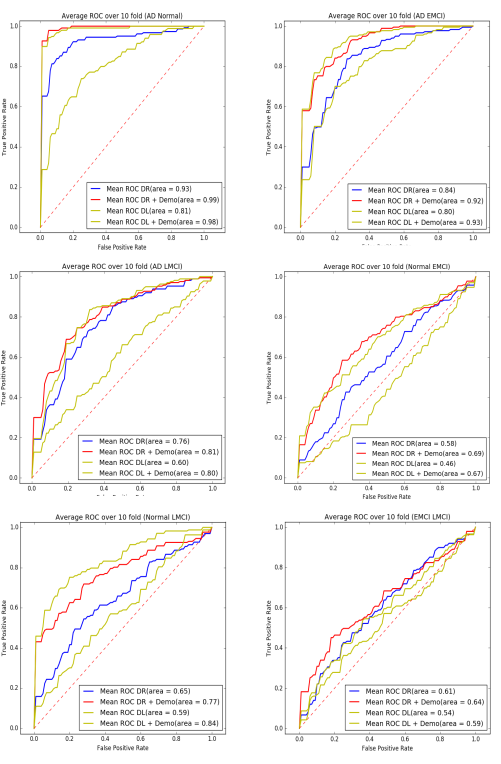
\includegraphics[width=0.9\linewidth]{figures/auc.png}
	\caption{ROC comparing all clinical groups}
	\label{fig:auc}
\end{figure}



\section{Discussion}
In this paper, we propose a new imaging prediciton system called patch based feature extraction for Alzheimer's disease diagnosis via FDG-PET analysis (PFE) for the early prediction of cognitive imparemet and diagnose AD and its various stages in progesssion (EMCI and LMCI). Deriving motivation from some prior work in surface morphmetry statistics  \citep{zhang2016applyiong,zhang2016hyperbolic}  we selected a series of different extent overlapped patches and applied max-pooling. For dimension redction, we selected a series of algorithms and performed meta analysis to determine the best performing one. We base our classifier as AdaBoost as it has proven to be a excellent choice for biomedical research  \citep{?.?}. The result on 663 baseline subjects from ADNI show that our PFE framework performed better than some other standard image measures. Our study has two main findings. First, the combined statistics for each subject, consting of APOE gene information, FAQ scores and other demographic features carries rich information on distributed metabolic activity, which measures volumetric deformation and are also applicable for prediction and classification research. The newly combined statistics practically encodes a great deal of information that would be otherwise overlooked, volumetric based computer-aided diagnostic research is more powerful by analysing these rich features. Second, we try to demonstrate the feasibility of learning algorithms in image based predicion and classification research. SCC is an efficient sparse coding algorithm and its superior computational efficiency helps us to account for biological differences and achieve deep learning.~\cite{gregor2010learning} pointed out that sparse coding is a special case of sparse encoder method  \citep{vincent2010stacked,baldi2012autoencoders}. These deep architectures have shown to lead to state-of-the-art results on a number of challenging classification and regression problem. We find out the the encoding of features involving volumetric data is large thus costly to impliment and there is no significant performance improvment in the training.  

\subsection{Methods for ADNI classification using PET subsectioncans}
The development of automatic methods for the accurate classification of patients into clinical groups from imaging data has been the aim of a number of ADNI studies. Thus PET classification plays an important role in medical image retrieval, which is a part of decision making in medical image analysis. ADNI 2 PET data is new compared to ADNI 1 and has two different modalities for traditional MCI i.e. EMCI and LMCI which are the early and late stages in imparement.

For 3D PET scans ``Z-score'' images are used to represent the active parts of the brain it will show all pixels with values below the lower threshold in blue, and pixels above the upper threshold in red \citep{ishii2014pet}. PET scans have also been analyzed by utilizing adjusted $T$ statistics and an automated voxel-based procedure \citep{herholz2002discrimination} and Machine Learning algorithms to address the high dimensionality of the statistical maps \citep{illan201118} \citep{higdon2004comparison}. Recently minor cognitive impairment (MCI) in \FDGPET ~has been classified by a brain regional sensitivity mapping method based on summated index (Total Z score) by utilizing the sensitivity-distribution maps \citep{kakimoto2011new}. In other contemporary works a region of interest (ROI) mask is used to extract features and use incomplete random forest-robust support vector machine to perform classification \citep{lu2017early}. In previous work within our lab MRI images were classified using surface measures of ventricular enlargement and sparse coding then applied on the 2D-patch features \citep*{zhang2016hyperbolic,zhang2016applying} with $ 96.7 \% $ accuracy. These images were functional MRIs and the features were a combination of surface statistics, we build our idea on a similar model we fist design a empirical machine learning based model. Using three dimensional patches (i.e., small sub volumes of the image defined as three-dimensional [3D] cubes) we extract information. A very similar 3D patch based feature selection is described in \citep{coupe2011patch}, In  this work, voxels  with  similar  surrounding  neighborhoods  are  considered  to  belong  to  the  same  structure and thus are used to estimate the final label. Our data is also along the same lines. 

\subsubsection{Finding Dictionary and Sparse Codes}
\label{sec:dictionary_learning}
Dictionary learning is widely used in machine learning, neuroscience, signal processing, and statistics. It is the learning of the basis set, also called the dictionary, to adapt it to specific data, an approach that has recently proven to be very effective for signal processing in the audio and image processing domains. Different from traditional feature extraction methods like principle component analysis and its variants, sparse coding learns non-orthogonal and over-complete dictionaries which have more flexibility to represent data. Stochastic Coordinate Coding has been used successfully in the past \citep{lin2014stochastic,mairal2009online}. 

Given a data set $\mathbf{X} = (x_1 \dots x_n)$ of image patches, each image patch is a {\em p}-dimensional vector i.e., $ x_i \in \mathbb{R}^{p} $, $ i = 1, \dots, n $. Specifically, suppose there are \emph{m} atoms $ \mathbf{d_j} \in \mathbb{R}, j = 1,\dots,m $, where the number of atoms is usually much smaller than the number of image patch {\em p}. Each patch can be represented as $ \mathbf{x_i} =  \sum^m_{j=1} z_{i,j}d_j $. In this way, the {\em p}-dimensional vector $ \mathbf{x_i} $ is represented by an m-dimensional vector $  \mathbf{z_i} = (z_{i,1},\dots,z_{1,m})^T $ which means the learned feature vector $ \mathbf{x_i} $ is a sparse vector. 

\begin{figure}
	\centering
	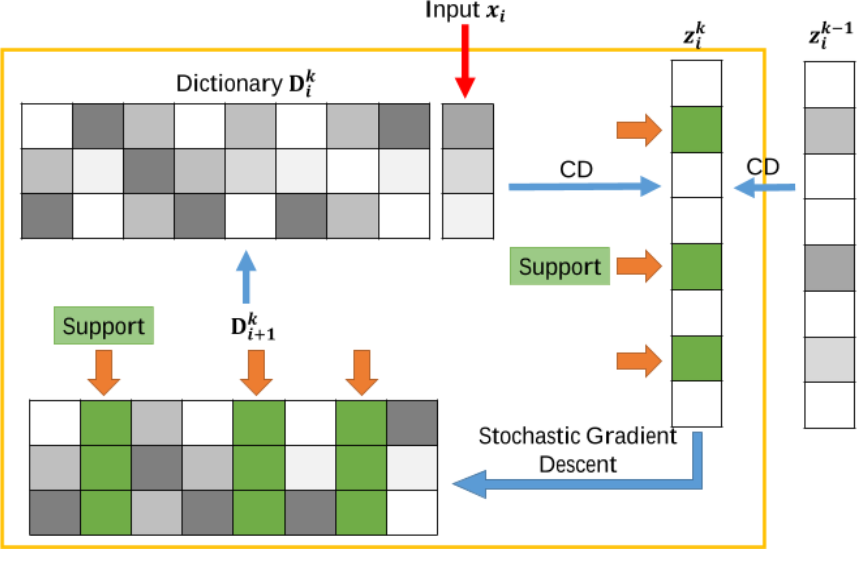
\includegraphics[width=\linewidth]{figures/iteration}
	\caption[One Iteration of SCC]{Figure shows one iteration of the sparse coding algorithm. (a).Take an image patch $x_i$. (b). Perform few steps of coordinate descent to find the support (non zero entries) of the sparse code. (c). Update the support of the dictionary by second order stochastic gradient descent to obtain a new dictionary.}
	\label{fig:iteration}
\end{figure}

As illustrated in Fig.~\ref{fig:iteration} shows the input $ x_i $ and the sparse vector $ z^k_i $ where i is the sample number and k is the iteration.


\begin{algorithm}
	\vspace{1em}
	\caption{Patch Based Stochastic Coordinate Coding}
	\label{alg:pipeline1}
	
	\KwIn{A number of FDG-PET images}
	
	\KwOut{A set of features and labels for the six classification experiment}
	
	The segmented dataset is divided and segregated into 6 binary parcels
	
	\For{exp $ \gets $ \{ [AD vs. CU], [AD vs. EMCI], [AD vs. LMCI], [CU vs. EMCI], [CU vs. LMCI], [EMCI vs. LMCI]. \}} {
		
		m $ \gets $ number of samples
		
		n $ \gets $ number of patches
		
		p $ \gets $ patch dimension
		
		Initialize X = [m*n $ \times $ p]
		\For{samples $ \in $ exp}{
			A three dimensional patch of 10 $ \times $ 10 $ \times $ 10 is created in order to extract meaning full information from the 3D segmented PET scans.   
		
	    	A number of random patches are generated over the volume and random meaningful patches are selected from the ROI to initialize the dictionary. 
	
			\For{patch $ \in $ patches}{
				 downsample ``patch'' \& linearly rearranged $ X_{patch} = (x_1,\dots,x_p)$ where $ patch \in p$.
			
				A matrix of all patches is arranged. i.e., X[sample*patch, : ] = [ $X_{patch}$']
			}
	}

	$ X $ is then fed into the stochastic coordinate coding module. (Fig. \ref{fig:pipeline1}(c)).
	
	We apply max-pooling algorithm on the learned 2000-dimension dictionary to aggregate discriminant features (Fig. \ref{fig:pipelinecompare}(d)).
	
	Ada-Boost is used to classify the six binary classification experiments. 
	}
\end{algorithm}


%\subsection{Selecting the best patch size}

\section{Conclusion and Future Work}
In this paper, we present a frameworks that combines three dimensional voxel statistics with machine learning to deal with high dimensional features before classification. We also used dictionary learning and sparse coding to study the effectiveness of leature learning algorithm with respect to the original framework. We applied AdaBoost to classify different AD stages. Our comprehensive experiments showed the effectiveness of patch based methods in three dimensional Positron Emission Tomography (PET). We obtained $ ~96 \% $ classification with voxel + demographic statistics.
Our proposed PFE method performs well in experiments with high group separation. With experiments having low group separation both the algorithms struggled. This indicates that there is significant metabolic change in AD vs. CU but in other stages the metabolic change may be unpredictable to some extent. 

We hope our work sheds light on the utilization of PET images as biomarker information in classifying Non-AD classes with a greater accuracy. It also invokes the use of varied multiple features in the diagnosis of Alzheimer's via some clinical group classification. In the future, we plan to apply our systems to other cortical and sub-cortical regions in the brain, more specifically to design a better ROI based feature selection method so as to identify regions in the cortex and sub-cortex responsible for cognitive decline.

\begin{center}
{\large Acknowledgements}
\end{center}

This work was partially supported by the National Institutes of Health (R21AG043760 to JS, WZ, RJC and YW, R21AG049216 to WZ and YW, RF1AG051710 and U54EB020403 to YW, R01AG031581 and P30AG19610 to RJC) and the National Science Foundation (DMS-1413417 to YW, IIS-1421165 to WZ and YW).

Data collection and sharing for this project was funded by the Alzheimer\textquoteright s Disease Neuroimaging Initiative (ADNI) (National Institutes of Health Grant U01 AG024904) and DOD ADNI (Department of Defense award number W81XWH-12-2-0012). ADNI is funded by the National Institute on Aging, the National Institute of Biomedical Imaging and Bioengineering, and through generous contributions from the following: Alzheimer's Association; Alzheimer\textquoteright s Drug Discovery Foundation; BioClinica, Inc.; Biogen Idec Inc.; Bristol-Myers Squibb Company; Eisai Inc.; Elan Pharmaceuticals, Inc.; Eli Lilly and Company; F. Hoffmann-La Roche Ltd and its affiliated company Genentech, Inc.; GE Healthcare; Innogenetics, N.V.; IXICO Ltd.; Janssen Alzheimer Immunotherapy Research \& Development, LLC.; Johnson \& Johnson Pharmaceutical Research \& Development LLC.; Medpace, Inc.; Merck \& Co., Inc.; Meso Scale Diagnostics, LLC.; NeuroRx Research; Novartis Pharmaceuticals Corporation; Pfizer Inc.; Piramal Imaging; Servier; Synarc Inc.; and Takeda Pharmaceutical Company. The Canadian Institutes of Health Research is providing funds to Rev December 5, 2013
support ADNI clinical sites in Canada. Private sector contributions are facilitated by the Foundation for the National Institutes of Health (www.fnih.org). The grantee organization is the Northern California Institute for Research and Education, and the study is coordinated by the Alzheimer\textquoteright s Disease Cooperative Study at the University of California, San Diego. ADNI data are disseminated by the Laboratory for Neuro Imaging at the University of Southern California.

\appendix
\subsection{\textbf{Stochastic Coordinate Coding}}
\label{app:SCC}
The following section describes Stochastic Coordinate Coding (SCC) algorithm \citep{lin2014stochastic}. The dictionary is initialized via any initialization method and denoted as $ D_1^1 $. The sparse codes are initialized as $ z_i^0 = 0 $ for $ i=1,\dots,n $. Where $ i $ is the index of data points and the superscript denotes the number of epoch. The algorithm is describes as follows:\\
(1). Get an image patch $ x_i $.\\
(2). Update $ z_i^k $ via one or a few steps of coordinate descent: 
\begin{equation}
z^k_i = CD(D^k_i,z^{k-1}_i,x_i).
\end{equation}
Specifically, for $ j $ from 1 to $ m $, update the $ j $-th coordinate $ z_{i,j}^{k-1} $ of $ z_{i}^{k-1} $ cyclically as follows:
\begin{equation}
b_j \gets (d_{i,j}^k)^T (x_i - D_i^kz^{k-1}_i) + z^{k-1}_{i,j}, z_{i,j}^{k-1} \gets h_{\lambda}(b_j),
\end{equation}	
where h is the soft thresholding shrinkage function. We call such cycle as one step of coordinate descent. The updated sparse code is then denoted by $ z_i^k $. \\
(3). Update the dictionary $ D $ by using stochastic gradient descent:
\begin{equation}
D_{i+1}^k = P_{B_m}(D_i^k - \eta^k_i\Delta_{D_i^k} f_i(D_i^k,z^k_i))
\end{equation}

where $ P $ denotes the projection operator. We set the learning rate as an approximate of the inverse of the Hessian matrix. The gradient of $ D_i^k $ can be obtained as follows:

\begin{equation}
\Delta_{D_i^k} f_i (D_i^k, z_i^k) = (D^k_iz^k_i - x_i)(z^k_i)^T.
\end{equation}

(4). $ i = i+1 $. If $ i \ge n $, then set $ D_1^{k+1} = D^k_{n+1}, ~k=k+1$ and $ i = 1 $.

When the data sets are very large, the learning rate $ \eta^k_i $ will be very small. In this case, the dictionary will not change very much and the efficiency of the training will decrease. In practice tuning the learning rate is tricky and sensitive. To obtain the learning rate we use the Hessian matrix of the objective function. It is shown that the following matrix provides an approximation of the Hessian: $ \mathbf{H} = \sum_{k,i} z^k_i(z^k_i)^T $, when $ k $ and $ i $ go to infinity. According to the second order stochastic gradient descent, we should use the inverse matrix of the Hessian as the learning rate. However, computing a matrix inversion problem is computationally expensive. In order to get the learning rate, we simply use the diagonal elements of the matrix $ H $. The matrix $ H $ is updated as follows:
\begin{equation}
	H \gets H + z^k_i(z^k_i)^T.
\end{equation}

Alg. \ref{alg:scc} summarizes the steps described in section \ref{sec:dictionary_learning}

\begin{algorithm}
	
	\caption{SCC (Stochastic Coordinate Coding)}\label{alg:scc}
	
	\KwIn{Data set $ X = (x_1,x_2,\dots,x_n) \in R^{p \times n} $, ensure $ D \in R^{p \times m} $ and $ Z =  (z_1 \dots z_n ) \in R ^{m \times n}$}
	\KwOut{$ D = D^k_n$ and $z_i = z_i^k $ for $ i = i,\dots,n $.}
	
	Initialize $ D_1^1, H = 0 $ and $ z_i^0 $ for $ i = 1,\dots,n $,
	
	\For{$ k = 1 $ to $ k $ do }
		{\For{$ i = 1$ to $ n $}
			{Get an image patch $ x_i $\\
			Update $ z_i^k $ via one or a few steps of coordinate descent: \hspace{1.5cm}$ z_i^k \gets CD(D_i^k,z^{k-1}_i,x_i)$.\\
			Update the Hessian matrix and the learninig rate:
			\hspace{1.5cm}$ H \gets H + z^k_i(z^k_i)^T, ~\eta^k_{i,j} = \frac{1}{h_{jj}} $.\\
			Update the support of the dictionary via SGD:
			\hspace{1.5cm}$ d^k_{i+1,j} \gets d^k_{i,j} - \eta^k_{i,j}z_{i,j}(D_i^kz^k_i - x_i) $\\
			If $ i = n $, set $ D_1^{k+1} = D^k_{n+1} $.
		}
		}
	
\end{algorithm}

\newpage

\begin{center}
{\large References}
\end{center}

\bibliographystyle{model2-names}
\bibliography{confinv}

\end{document}

